\newpage
\ifthenelse {\boolean{bachelor}}
{
	%\section{Analysis}
	\section{Analýza} 
}
{
	%\chapter{Analysis}
	\chapter{Analyza}
}
V tejto kapitole priblížím a rozoberiem čo je spracovanie prirodzeného jazyka, kde a ako sa dá využiť. Ďalej zanalyzujem existujúce aplikácie a systému, ktorých základom je spracovanie textu.
\ifthenelse {\boolean{bachelor}}
{
	%\subsection{Subsection}
	\subsection{Spracovanie prirodzeného jazyka}
}
{
	%\section{Subsection}
	\section{Spracovanie prirodzeného jazyka}
}
\label{subsec:nlp}
Spracovanie prirodzeného jazyka (angl. Natural Language Processing - NLP) je oblasť vedného oboru, ktorý sa zaoberá počítačovými technológiami. Hlavným cieľom NLP je dosiahnuť aby počítač dokázal porozumieť ľudskej, či už písanej alebo hovorovej, reči.

Porozumenie ľudskej reči je mnohokrát náročne aj pre samotných ľudí a nie to ešte pre počítače. Na svete je veľké množstvo jazykov, ktoré sa od seba líšia charakteristikami typickými pre konkrétny jazyk. Taktiež každý človek sa líši a preto výslovnosť rovnakého slova viacerými ľuďmi môže byť odlišná. Ďalej máme slangové slová a slová typické len pre určité územie. Pri spracovávaní prirodzeného jazyka treba vziať do úvahy tieto a aj ďalšie premenné. Dosiahnutie tohto cieľa je preto často veľmi náročné.

V súčastnosti najpoužívanejšie algoritmy na NLP využívajú strojové učenie. Dosiahnutie úplného porozumenia a spracovania ľudského prirodzeného jazyka by znamenalo vyriešiť \textit{AI-complete} problém, čo znamená, že obtiažnosť tohto problému je ekvivalentné z obtiažnosti problému vytvorenia počítača inteligentného ako človek, takzvané ,,true AI''.

NLP ma niekoľko hlavných úloh. Podrobnejšie si priblížime tie, ktoré sú relevantné vzhľadom na implementáciu spracovania učebných textov.

Úlohy spracovania prirodzeného textu: [Natural Language Processing (Almost) from Scratch, Ronan Collobert]
\begin{itemize}
	\item Značkovanie slovných druhov (angl. Part-of-speech tagging) \ref{subsubsec:postagging}
	\item Rozdelenie vety na menšie časti (angl. Chunking)
	\item Rozpoznávanie názvoslovných entít (angl. Named Entity Recognition) \ref{subsubsec:ner}
	\item Označovanie sémantického postavenie (angl. Semantic Role Labeling)
	\item Rozpoznanie koreferencií (angl. Coreference resolution) \ref{subsubsec:corefparsing}
	\item Morfologické segmentovanie (angl. Morphological Segmentation)
	\item Generovanie prirodzeného jazyka (angl. Natural Language Generation)
	\item Optické rozoznávanie textu (angl. Optical Character Recognition)
	\item Rozloženie vzťahov (angl. Dependency parsing) \ref{subsubsec:corefparsing}
	\item a mnoho ďalších
\end{itemize}

\ifthenelse {\boolean{bachelor}}
{
	%\subsection{Subsection}
	\subsubsection{Značkovanie slovných druhov}
}
{
	%\section{Subsection}
	\subsection{Značkovanie slovných druhov}
}
\label{subsubsec:postagging}
Hlavnou úlohou značkovania slovných druhom (angl. Part-of-speech tagging) je každému slovu vo vete priradiť unikátnu značku, ktorá odrážať jeho syntaktickú úlohu vo vete. Sú to, napríklad v slovenskom jazyku podmet, prísudok, príslovkové určenie alebo v anglickom jazyku noun, adverb, verb, atď. Tak isto to môže byť označenie určujúce množné číslo, napríklad signulár alebo plurál.

Problémom pri značkovaní slovných druhov je mnohoznačnosť. Znamená to, že slovo môže mať viacero významov a môže byť viacerými slovnými druhmi. Napríklad v slovenskom jazyku slovo \textit{kry} môže predstavovať sloveso s významom rozkazu \textit{prikry!}, ale taktiež môže predstavovať podstatné meno s významom \textit{kríky}. V anglickom jazyku to je napríklad slovo \textit{book}, ktoré môže predstavovať podstatné meno (angl. noun) \textit{kniha} alebo sloveso (angl. verb) vo význame \textit{rezervovať}.

\ifthenelse {\boolean{bachelor}}
{
	%\subsection{Subsection}
	\subsubsection{Rozpoznávanie názvoslovných entít}
}
{
	%\section{Subsection}
	\subsection{Rozpoznávanie názvoslovných entít}
}
\label{subsubsec:ner}
Rozpoznávanie názvoslovných entít (angl. Named Entity Recognition) označuje mená a názvy, ktoré sa vyskytujú v texte. Rozdeľuje tieto entity do kategórií, ako sú napríklad \textit{osoby}, \textit{organizácie} alebo \textit{lokácie}.

Ťažkosti pri rozpoznávaní názvoslovných entít spôsobuje kapitalizácia slov, takzvané písanie entít s veľkým začiatočným písmenom. V anglickom jazyku to jednoduché, kedže v angličtine sa entity píšu s veľkým začiatočným písmenom. Príklad je \textit{Slovak University of Technology}. Avšak v iných jazykoch to neplatí a entity sa nemusia písať s veľkým začiatočným písmenom.

\ifthenelse {\boolean{bachelor}}
{
	%\subsection{Subsection}
	\subsubsection{Rozpoznanie koreferencií}
}
{
	%\section{Subsection}
	\subsection{Rozpoznanie koreferencií}
}
\label{subsubsec:corefparsing}
Nájdenie, identifikácia a rozpoznanie koreferencií v texte je úlohou rozpoznávania koreferencií (angl. Coreference resolution). V texte sa často používajú zámena (angl. pronouns) \textit{to}, \textit{tí}, \textit{on} alebo anglicky \textit{it}, \textit{those}, \textit{he} a mnoho ďalších. Tieto zámena sa odkazujú na iné podstatné mená alebo mená a názvy a je úlohou rozpoznávania koreferencií určiť, na ktoré podstatné meno alebo meno, alebo názov sa konkrétne zámeno odkazuje.

Príklad:
\textbf{Martin Nemček} napísal túto bakalársku prácu. \textbf{On} študuje na FIIT STU BA.

Tu je vidno, že zámeno \textit{on} sa odkazuje na meno \textit{Martin Nemček}.

\ifthenelse {\boolean{bachelor}}
{
	%\subsection{Subsection}
	\subsubsection{Rozloženie vzťahov}
}
{
	%\section{Subsection}
	\subsection{Rozloženie vzťahov}
}
\label{subsubsec:dependencyparsing}
Dummy text..


\begin{figure}[H]
\begin{center}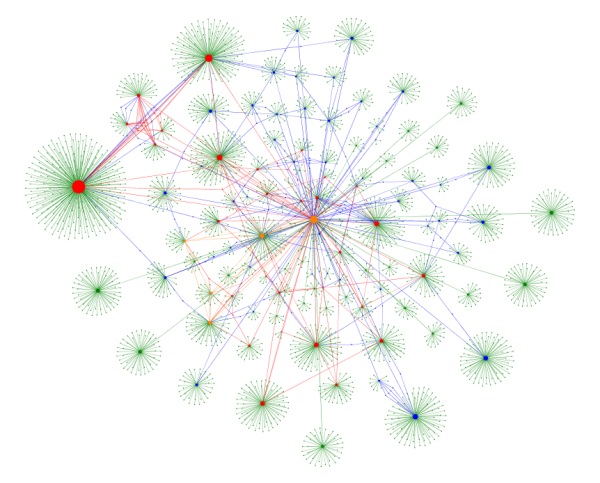
\includegraphics[scale=0.48]{figure}\end{center}
\caption[Name figure]{Name figure}\label{fig:figure}
\end{figure}
\subsection{Enumeration}
%\subsection{Číslovaný zoznam}
\begin{my_enumerate}
	\item {goal 1}
	\begin{my_enumerate}
		\item {goal 1.a}
		\item {goal 1.b}
	\end{my_enumerate}
	\item {goal 2}
	\item {goal 3}
\end{my_enumerate}
\subsection{Itemization}
%\subsection{Zoznam}
\begin{my_itemize}
	\item {item 1}
	\begin{my_itemize}
		\item {item 1.1}
		\item {item 1.2}
	\end{my_itemize}
	\item {item 2}
	\item {item 3}
\end{my_itemize}
\subsection{Citation}
%\subsection{Citácia}
Lorem ipsum dolor sit amet, consectetuer adipiscing elit, sed diam nonummy nibh euismod tincidunt ut laoreet dolore magna aliquam erat volutpat~\cite{1}.

\subsection{Labesl \& References}
%\subsection{Návestia \& Referencie}
See Section~\ref{lab:Examples}.

\subsection{Examples}
%\subsection{Príklady}
\label{lab:Examples}

\begin{lstlisting}[ language=html, caption={Example 1}, label={metrics_LOC},
	keywordstyle=\color{blue}\bfseries,
	ndkeywordstyle=\color{black}\bfseries,
	commentstyle=\color{red}\ttfamily,
	stringstyle=\color{green}\ttfamily,
	identifierstyle=\color{gray},
	backgroundcolor=\color{white}, 
	frame=single, 
	frameround=ffff,
	captionpos=b,
	basicstyle=\scriptsize
	]
<table class="metric_index">
	<tr>
		<th>Lines of code</th>
		<th>Value</th>
	</tr>
	<% if (filenum and modulenum) then %>
		<tr>
			<td class="name">Number of files</td>
			<td class="value"><%=filenum%></td>
		</tr>
		<tr>
			<td class="name">Number of modules</td>
			<td class="value"><%=modulenum%></td>
		</tr>
		<tr>
	<% end %>
	<tr>
		<td class="name">Lines Total</td>
		<td class="value"><%=LOC.lines%></td>
	</tr>
	<!--
							skryty zdrojovy kod
		podobne zobrazenie ostatnych metrik riadkov
	-->
</table>
\end{lstlisting}

\begin{lstlisting}[language=lua, caption={Názov}, label=metrics.pipe]
local parser  = require 'leg.parser'
local rules = require 'metrics.rules'
-- << skryty zdrojovy kod >> --
local capture_table = {}
grammar.pipe(LOC_capt.captures, AST_capt.captures)
grammar.pipe(block_capt.captures, LOC_capt.captures)
-- << viacero rovnakych volani s tabulkami captures inych modulov >> --
grammar.pipe(capture_table, cyclo_capt.captures)
local lua = lpeg.P(grammar.apply(parser.rules, rules.rules, capture_table))
local patt = lua / function(...) 
	return {...} 
end
local result = patt:match(code)[1]
\end{lstlisting}
